\documentclass[tikz]{standalone}
\usepackage{amsmath}
\usetikzlibrary{calc}
\definecolor{bg}{HTML}{171D2B}
\definecolor{accent}{HTML}{F7B538}
\begin{document}
\pagecolor{bg}
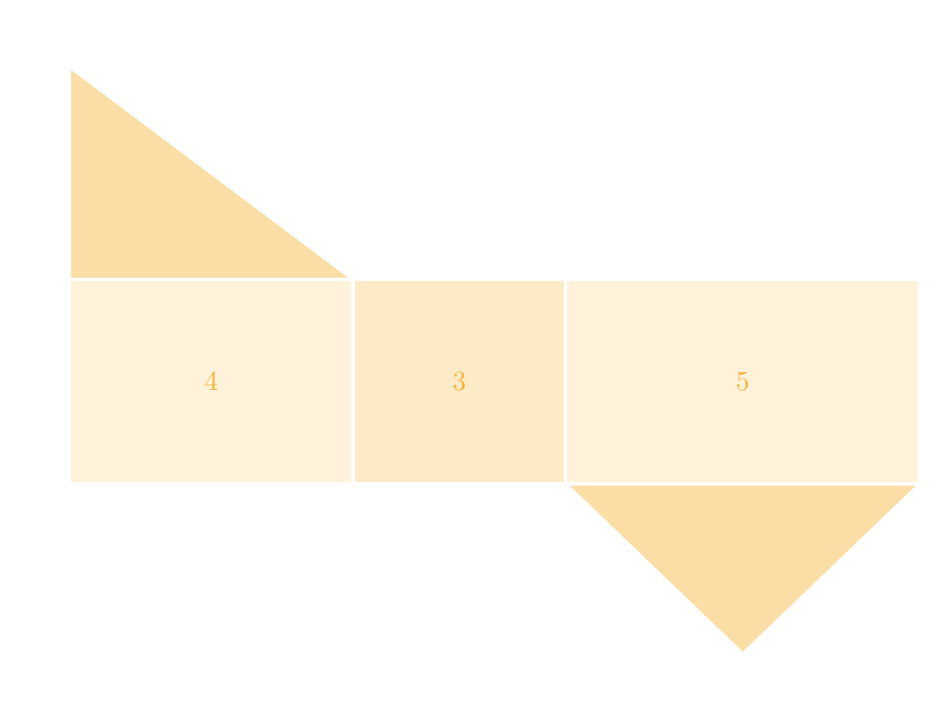
\begin{tikzpicture}[line width=1.2pt]
  \color{white}
  % Layout strip klasik: tiga persegi panjang berdampingan (lebar = panjang rusuk
  % alas 4, 3, 5), segitiga kongruen menempel di atas dan di bawah strip.
  \def\sx{0.9}  % skala cm per satuan
  \def\h{2.6}   % tinggi prisma
  \pgfmathsetmacro{\ua}{4*\sx}  % rusuk AB
  \pgfmathsetmacro{\ub}{3*\sx}  % rusuk AC
  \pgfmathsetmacro{\uc}{5*\sx}  % rusuk BC
  % x-offsets strip
  \def\xa{0}
  \pgfmathsetmacro{\xb}{\ua}
  \pgfmathsetmacro{\xc}{\ua+\ub}
  \pgfmathsetmacro{\xd}{\ua+\ub+\uc}
  % strip persegi panjang
  \draw[fill=accent!18, draw=white] (\xa,0) rectangle (\xb,\h);
  \draw[fill=accent!28, draw=white] (\xb,0) rectangle (\xc,\h);
  \draw[fill=accent!18, draw=white] (\xc,0) rectangle (\xd,\h);
  % segitiga atas: kongruen ABC, alas AB=4 di atas strip pertama
  \draw[fill=accent!45, draw=white] (\xa,\h) -- (\xb,\h) -- (\xa,\h+3*\sx) -- cycle;
  \node[above left]  at (\xa,\h+3*\sx) {\color{white}$C$};
  \node[below left]  at (\xa,\h) {\color{white}$A$};
  \node[above right] at (\xb,\h) {\color{white}$B$};
  % segitiga bawah: kongruen, alas BC=5 di bawah strip ketiga; tinggi dari BC = 12/5
  \pgfmathsetmacro{\hb}{12/5*\sx}
  \draw[fill=accent!45, draw=white] (\xc,0) -- (\xd,0) -- ({\xc+0.5*\uc},-\hb) -- cycle;
  \node[below] at ({\xc+0.5*\uc},-\hb) {\color{white}pasangan $ABC$};
  % label rusuk di strip
  \node[accent] at ({0.5*\xa+0.5*\xb},\h/2) {\color{accent}$4$};
  \node[accent] at ({0.5*\xb+0.5*\xc},\h/2) {\color{accent}$3$};
  \node[accent] at ({0.5*\xc+0.5*\xd},\h/2) {\color{accent}$5$};
\end{tikzpicture}
\end{document}
